\documentclass[12pt,a4paper]{article}
\usepackage[utf8]{inputenc}
\usepackage[T1]{fontenc}
\usepackage{geometry}
\usepackage{graphicx}
\usepackage{fancyhdr}
\usepackage{titlesec}
\usepackage{amsmath}
\usepackage{amsfonts}
\usepackage{amssymb}
\usepackage{booktabs}
\usepackage{longtable}
\usepackage{array}
\usepackage{multirow}
\usepackage{multicol}
\usepackage{xcolor}
\usepackage{colortbl}
\usepackage{tikz}
\usepackage{pgfplots}
\usepackage{forest}
\usepackage{hyperref}
\usepackage{enumitem}
\usepackage{float}
\usepackage{caption}
\usepackage{subcaption}
\usepackage{listings}
\usepackage{textcomp}
\usepackage{gensymb}
\usepackage{siunitx}
\usepackage{acronym}
\usepackage{glossaries}
\usepackage{pdfpages}
\usepackage{rotating}
\usepackage{pdflscape}
\usepackage{afterpage}
\usepackage{placeins}

% Page geometry
\geometry{
    left=2.5cm,
    right=2.5cm,
    top=2.5cm,
    bottom=2.5cm,
    headheight=1.5cm,
    headsep=0.5cm,
    footskip=1cm
}

% Colors
\definecolor{spitblue}{RGB}{0,51,102}
\definecolor{spitgold}{RGB}{255,204,0}
\definecolor{darkblue}{RGB}{0,31,63}
\definecolor{lightblue}{RGB}{173,216,230}
\definecolor{gray}{RGB}{128,128,128}

% Hyperref settings
\hypersetup{
    colorlinks=true,
    linkcolor=spitblue,
    filecolor=spitblue,
    urlcolor=spitblue,
    citecolor=spitblue,
    pdftitle={AEGIS: Advanced Enterprise Grid \& Industrial Security Platform},
    pdfauthor={Bharatiya Vidya Bhavan's Sardar Patel Institute of Technology},
    pdfsubject={Government Research Proposal},
    pdfkeywords={Cybersecurity, OT Security, Industrial Control Systems, Smart Grid}
}

% Header and footer
\pagestyle{fancy}
\fancyhf{}
\fancyhead[L]{
\includegraphics[width=2cm]{spit_logo.png}}
\fancyhead[C]{\textbf{\footnotesize AEGIS Research Proposal}}
\fancyhead[R]{\footnotesize Page \thepage}
\fancyfoot[C]{\footnotesize Bharatiya Vidya Bhavan's Sardar Patel Institute of Technology}
\renewcommand{\headrulewidth}{0.4pt}
\renewcommand{\footrulewidth}{0.4pt}

% Title formatting
\titleformat{\section}
{\color{spitblue}\normalfont\Large\bfseries}
{\color{spitblue}\thesection}{1em}{}

\titleformat{\subsection}
{\color{darkblue}\normalfont\large\bfseries}
{\color{darkblue}\thesubsection}{1em}{}

\titleformat{\subsubsection}
{\color{darkblue}\normalfont\normalsize\bfseries}
{\color{darkblue}\thesubsubsection}{1em}{}

% Custom commands
\newcommand{\rupees}{₹\,}
\newcommand{\crores}{\text{ Crores}}
\newcommand{\lakhs}{\text{ Lakhs}}

% Table settings
\renewcommand{\arraystretch}{1.3}

% Listings settings for code
\lstset{
    basicstyle=\ttfamily\footnotesize,
    breaklines=true,
    frame=single,
    numbers=left,
    numberstyle=\tiny,
    tabsize=2,
    showspaces=false,
    showstringspaces=false
}

% Glossary
\makeglossaries
\newacronym{ot}{OT}{Operational Technology}
\newacronym{it}{IT}{Information Technology}
\newacronym{ics}{ICS}{Industrial Control Systems}
\newacronym{scada}{SCADA}{Supervisory Control and Data Acquisition}
\newacronym{ai}{AI}{Artificial Intelligence}
\newacronym{ml}{ML}{Machine Learning}
\newacronym{soc}{SOC}{Security Operations Center}
\newacronym{siem}{SIEM}{Security Information and Event Management}
\newacronym{iiot}{IIoT}{Industrial Internet of Things}

\begin{document}

% Title page
\begin{titlepage}
    \centering
    
    % Logo
    \vspace*{-1cm}
    
\includegraphics[width=4cm]{spit_logo.png}
    
    \vspace{1cm}
    
    {\Large\textbf{BHARATIYA VIDYA BHAVAN'S}\\[0.2cm]}
    {\Large\textbf{SARDAR PATEL INSTITUTE OF TECHNOLOGY}\\[0.3cm]}
    {\normalsize Munshi Nagar, Andheri (West), Mumbai - 400058, Maharashtra, India\\[0.5cm]}
    
    \vspace{1cm}
    
    % Title
    {\color{spitblue}\Huge\textbf{AEGIS}}\\[0.5cm]
    {\color{darkblue}\Large\textbf{Advanced Enterprise Grid \& Industrial Security Platform}}\\[0.3cm]
    {\large A Next-Generation Distributed OT/IT Cybersecurity Ecosystem}\\[1cm]
    
    % Subtitle
    {\color{spitblue}\Large\textbf{PROFORMA FOR SUBMITTING R\&D PROJECT PROPOSAL}}\\[0.3cm]
    {\color{spitblue}\Large\textbf{FOR SEEKING FINANCIAL SUPPORT}}\\[1.5cm]
    
    % Project details box
    \begin{center}
    \fbox{\begin{minipage}{0.8\textwidth}
        \centering
        \textbf{Project Codename:} AEGIS\\[0.2cm]
        \textbf{Total Budget:} \rupees 4,70,00,000 (4.7 Crores)\\[0.2cm]
        \textbf{Duration:} 36 Months\\[0.2cm]
        \textbf{Proposal Date:} \today\\[0.2cm]
        \textbf{Classification:} Strategic National Infrastructure Protection Initiative
    \end{minipage}}
    \end{center}
    
    \vfill
    
    % Bottom information
    {\large\textbf{Submitted to:} Government of India\\[0.2cm]}
    {\normalsize Under the National Cybersecurity Research Initiative\\[0.2cm]}
    {\normalsize for Critical Infrastructure Protection}
    
    \vspace{1cm}
    
    {\footnotesize Document Version: 3.0 Enhanced | Classification: Confidential - Government Use Only}
    
\end{titlepage}

\newpage

% Table of Contents
\tableofcontents
\newpage

% List of Figures
\listoffigures
\newpage

% List of Tables
\listoftables
\newpage

% Acronyms
\printglossary[type=\acronymtype,title=List of Acronyms]
\newpage

% Executive Summary
\section{Executive Summary}

The AEGIS (Advanced Enterprise Grid \& Industrial Security) platform represents a paradigm shift in industrial cybersecurity, introducing revolutionary concepts including quantum-resistant encryption, AI-driven predictive maintenance, zero-trust architecture for OT networks, and the world's first blockchain-verified industrial protocol analyzer. This comprehensive solution addresses the critical gap in India's industrial cybersecurity infrastructure while establishing the nation as a global leader in OT/IT security innovation.

\subsection{Strategic Value Propositions}
\begin{itemize}[leftmargin=*]
    \item \textbf{National Security Enhancement:} 99.99\% threat detection with zero-day exploit protection
    \item \textbf{Economic Impact:} Projected savings of \rupees 500\crores\ annually from prevented cyber incidents
    \item \textbf{Technology Leadership:} 15+ patent-worthy innovations in industrial cybersecurity
    \item \textbf{Workforce Development:} Creating 500+ specialized cybersecurity jobs
    \item \textbf{Export Potential:} \rupees 1000\crores\ export opportunity to friendly nations
\end{itemize}

% Summary Sheet as per Government Template
\section{PROFORMA SUMMARY SHEET}

\begin{longtable}{|p{3cm}|p{12cm}|}
\hline
\rowcolor{lightblue}
\textbf{Field} & \textbf{Details} \\
\hline
\endhead

\textbf{1. Title of Project} & 
AEGIS: Advanced Enterprise Grid \& Industrial Security Platform - A Next-Generation Distributed OT/IT Cybersecurity Ecosystem \\
\hline

\multirow{3}{*}{\textbf{2. Organisation}} & 
\textbf{a) Name:} Bharatiya Vidya Bhavan's Sardar Patel Institute of Technology (SPIT) \\
& \textbf{b) Address:} Munshi Nagar, Andheri (West), Mumbai - 400058, Maharashtra, India \\
& \textbf{c) Legal Status:} Autonomous Institute under Bharatiya Vidya Bhavan, Registered Trust \\
\hline

\multirow{4}{*}{\textbf{3. Chief Investigator}} & 
\textbf{a) Name:} Dr. [To be appointed - Senior Professor] \\
& \textbf{b) Designation:} Principal Investigator \& Head, Cybersecurity Research \\
& \textbf{c) Department:} Electronics \& Telecommunications Engineering \\
& \textbf{d) Address:} SPIT, Munshi Nagar, Andheri (West), Mumbai - 400058 \\
\hline

\textbf{4. Nature of Project} & 
\textbf{✓ a) Research, Development \& Engineering (R,D \& E) leading to production capability}\\
\textbf{✓ b) Application oriented Research, Design and Development (R,D\&D) having production potential}\\
c) Basic R\&D \\
\hline

\textbf{5. Objective of the Project} & 
\textbf{Primary Objectives:}
\begin{itemize}[leftmargin=1em]
    \item Develop indigenous distributed OT/IT cybersecurity platform
    \item Implement quantum-resistant encryption for industrial protocols
    \item Create AI-powered threat detection with 99.5\% accuracy
    \item Build blockchain-based forensic audit system
    \item Design hardware data diode for air-gapped security
    \item Establish comprehensive protocol support (50+ protocols)
    \item Develop real-time visualization and monitoring system
    \item Create automated incident response framework
\end{itemize} \\
\hline

\end{longtable}

\begin{longtable}{|p{3cm}|p{12cm}|}
\hline
\rowcolor{lightblue}
\textbf{Field} & \textbf{Details} \\
\hline
\endhead

\textbf{6. Brief outline with technology fall-outs} & 
\textbf{Coverage:} Complete OT/IT cybersecurity ecosystem with 8 integrated modules:
\begin{enumerate}[leftmargin=1em]
    \item AssetGuard - Intelligent Asset Discovery Engine
    \item ProtoSense - Universal Protocol Intelligence Platform  
    \item ThreatHunter - AI-Powered Threat Detection System
    \item ChainAudit - Blockchain-Powered Forensic System
    \item DiodeGuard - Hardware-Accelerated Data Diode
    \item VizDash - Advanced Visualization \& Command Center
    \item LogMiner - Intelligent Log Processing System
    \item AlertStream - Incident Response Orchestrator
\end{enumerate}

\textbf{Technology Fall-outs:}
\begin{itemize}[leftmargin=1em]
    \item Quantum-resistant cryptographic algorithms
    \item Industrial AI/ML models for anomaly detection
    \item Custom FPGA-based protocol parsers
    \item Blockchain-based audit trail system
    \item Zero-trust architecture for OT networks
    \item Custom hardware data diode design
    \item Real-time 3D network visualization
    \item Automated playbook execution engine
\end{itemize} \\
\hline

\multirow{3}{*}{\textbf{7. Expected outcome}} & 
\textbf{a) System Specifications:}
- Throughput: 1M events/sec, Latency: <100ms
- Protocol Support: 50+ industrial protocols
- Scalability: 10,000+ devices per deployment
- Availability: 99.99\% uptime with redundancy

\textbf{b) Technology Transfer Documents:}
- 15+ patents filed, Complete source code
- Technical documentation (1000+ pages)
- Training manuals and certification programs

\textbf{c) Manpower Training:}
- Level: Graduate/Post-graduate engineers, Industry professionals
- Numbers: 100 internal, 200 industry, 300 external participants \\
\hline

\textbf{8. Linkup Agency} & 
\textbf{Established Partnerships:}
\begin{itemize}[leftmargin=1em]
    \item Power Grid Corporation of India (POWERGRID)
    \item Indian Computer Emergency Response Team (CERT-In)
    \item National Critical Information Infrastructure Protection Centre (NCIIPC)
    \item Centre for Development of Advanced Computing (C-DAC)
    \item Defence Research and Development Organisation (DRDO)
\end{itemize}

\textbf{Proposed International Partnerships:}
\begin{itemize}[leftmargin=1em]
    \item SANS Institute (Training \& Certification)
    \item NIST (Standards Development)
    \item European Network and Information Security Agency (ENISA)
\end{itemize} \\
\hline

\textbf{9. Duration} & 36 Months (3 Years) \\
\hline

\end{longtable}

\newpage

% Year-wise milestones table
\begin{longtable}{|p{2cm}|p{4cm}|p{8cm}|}
\hline
\rowcolor{lightblue}
\textbf{Year} & \textbf{Phase} & \textbf{Physical Achievements \& Milestones} \\
\hline
\endhead

\multirow{4}{*}{\textbf{Year 1}} & Foundation & 
- Team recruitment (60+ experts)
- Infrastructure setup (₹80\lakhs)
- Test lab establishment
- Protocol analysis framework (10 protocols)
- AssetGuard alpha version
- Initial security framework design \\
\cline{2-3}
& Development & 
- ProtoSense parser development
- ThreatHunter ML model training
- DiodeGuard hardware prototype
- ChainAudit blockchain integration \\
\hline

\multirow{4}{*}{\textbf{Year 2}} & Core Development & 
- Complete protocol support (50+ protocols)
- AI/ML model optimization (95\% accuracy)
- VizDash 3D visualization system
- LogMiner analytics engine
- System integration framework \\
\cline{2-3}
& Advanced Features & 
- Quantum-resistant encryption implementation
- Zero-trust architecture deployment
- AlertStream automation engine
- Beta testing with pilot customers \\
\hline

\multirow{4}{*}{\textbf{Year 3}} & Integration \& Testing & 
- Full system integration testing
- Security audit \& penetration testing
- Performance optimization (1M events/sec)
- User acceptance testing \\
\cline{2-3}
& Deployment & 
- Pilot deployments (5 sites)
- Documentation completion (1000+ pages)
- Training program delivery (600+ participants)
- Patent filing \& IP protection \\
\hline

\end{longtable}

\begin{longtable}{|p{3cm}|p{12cm}|}
\hline
\rowcolor{lightblue}
\textbf{Field} & \textbf{Details} \\
\hline
\endhead

\textbf{11. Likely End Users} & 
\textbf{Primary End Users:}
\begin{itemize}[leftmargin=1em]
    \item Power Grid Corporation of India \& State Electricity Boards
    \item Oil \& Natural Gas Corporation (ONGC) \& Indian Oil Corporation (IOC)
    \item Nuclear Power Corporation of India (NPCIL)
    \item Indian Railways \& Metro Rail Corporations
    \item Smart City Mission Projects (100+ cities)
    \item Defence Establishments \& Strategic Industries
    \item Water Treatment \& Distribution Utilities
    \item Manufacturing Industries (Steel, Petrochemical, Pharma)
\end{itemize}

\textbf{Secondary Markets:}
\begin{itemize}[leftmargin=1em]
    \item International clients in friendly nations
    \item Private industrial enterprises
    \item Critical infrastructure in BRICS countries
    \item Cybersecurity service providers
\end{itemize} \\
\hline

\textbf{12. Joint Participants} & 
\textbf{Domestic Partners:}
\begin{itemize}[leftmargin=1em]
    \item Indian Institute of Technology (IIT) Delhi - AI/ML Research
    \item Indian Institute of Science (IISc) Bangalore - Quantum Computing
    \item Centre for Development of Advanced Computing (C-DAC) - HPC Integration
    \item Tata Consultancy Services (TCS) - System Integration
    \item Larsen \& Toubro (L\&T) - Hardware Manufacturing
    \item Bharti Airtel - Network Infrastructure
\end{itemize}

\textbf{International Collaborations:}
\begin{itemize}[leftmargin=1em]
    \item Carnegie Mellon University, USA - ICS Security Research
    \item Technical University of Denmark - Smart Grid Security
    \item Fraunhofer Institute, Germany - Industrial Cybersecurity
    \item National Institute of Standards and Technology (NIST), USA
\end{itemize} \\
\hline

\end{longtable}

\newpage

% Enhanced Budget Table
\section{DETAILED BUDGET BREAKDOWN}

\begin{table}[H]
\centering
\caption{Total Project Budget - 3 Year Breakdown (\rupees in Lakhs)}
\renewcommand{\arraystretch}{1.5}
\begin{tabular}{|p{3.5cm}|c|c|c|c|}
\hline
\rowcolor{lightblue}
\textbf{Budget Head} & \textbf{Year 1} & \textbf{Year 2} & \textbf{Year 3} & \textbf{Total} \\
\hline

\textbf{Capital Equipment} & 80.0 & 60.0 & 40.0 & \textbf{180.0} \\
\hline

\textbf{Consumable Stores} & 15.0 & 12.0 & 8.0 & \textbf{35.0} \\
\hline

\textbf{Manpower} & 80.0 & 70.0 & 60.0 & \textbf{210.0} \\
\hline

\textbf{Travel \& Training} & 8.0 & 7.0 & 5.0 & \textbf{20.0} \\
\hline

\textbf{Contingencies \& TA/DA} & 5.0 & 4.0 & 3.0 & \textbf{12.0} \\
\hline

\textbf{Overheads (10\%)} & 12.0 & 10.0 & 8.0 & \textbf{30.0} \\
\hline

\rowcolor{yellow}
\textbf{GRAND TOTAL} & \textbf{200.0} & \textbf{163.0} & \textbf{124.0} & \textbf{487.0} \\
\hline

\end{tabular}
\end{table}

\subsection{Detailed Capital Equipment Budget}

\begin{longtable}{|p{4cm}|p{6cm}|c|c|c|}
\hline
\rowcolor{lightblue}
\textbf{Equipment Category} & \textbf{Specification} & \textbf{Qty} & \textbf{Unit Cost} & \textbf{Total Cost} \\
& & & \textbf{(\rupees Lakhs)} & \textbf{(\rupees Lakhs)} \\
\hline
\endhead

\multicolumn{5}{|c|}{\cellcolor{gray}\textbf{HIGH-END COMPUTING INFRASTRUCTURE}} \\
\hline

\textbf{GPU Servers} & 
NVIDIA DGX A100 Systems
- 8x A100 80GB GPUs
- 1TB System RAM  
- 30TB NVMe Storage & 4 & 50.0 & 200.0 \\
\hline

\textbf{Compute Servers} & 
Dell PowerEdge R750
- 2x AMD EPYC 7763 (128 cores)
- 1TB RAM, 100TB NVMe SSD & 10 & 15.0 & 150.0 \\
\hline

\textbf{Storage Systems} & 
NetApp AFF A800
- 1PB usable all-flash storage
- 25GbE connectivity & 1 & 120.0 & 120.0 \\
\hline

\textbf{Network Infrastructure} & 
Cisco Nexus 9500 Series
- 400GbE capability
- 64 ports with redundancy & 2 & 40.0 & 80.0 \\
\hline

\multicolumn{5}{|c|}{\cellcolor{gray}\textbf{SPECIALIZED SECURITY HARDWARE}} \\
\hline

\textbf{Hardware Security Modules} & 
Thales Luna Network HSM
- FIPS 140-2 Level 3
- High-performance crypto & 2 & 20.0 & 40.0 \\
\hline

\textbf{Custom Data Diodes} & 
FPGA-based Hardware Design
- 10Gbps optical isolation
- Protocol validation & 4 & 15.0 & 60.0 \\
\hline

\multicolumn{5}{|c|}{\cellcolor{gray}\textbf{INDUSTRIAL CONTROL SYSTEMS TEST LAB}} \\
\hline

\textbf{Programmable Logic Controllers} & 
Siemens S7-1500 Advanced
- Safety-rated controllers
- Industrial Ethernet & 10 & 3.0 & 30.0 \\
\hline

\textbf{Remote Terminal Units} & 
SEL-3530 RTAC
- IEC 61850, DNP3 support
- Cybersecurity features & 8 & 3.0 & 24.0 \\
\hline

\textbf{Smart Meters} & 
Landis+Gyr E360
- 3-phase, AMI enabled
- Advanced security features & 100 & 0.2 & 20.0 \\
\hline

\textbf{Phasor Measurement Units} & 
SEL-421 Protection Relay
- IEEE C37.118 compliance
- Synchrophasor capability & 5 & 3.0 & 15.0 \\
\hline

\textbf{Power System Simulators} & 
OPAL-RT OP5700
- Real-time digital simulators
- Hardware-in-the-loop testing & 2 & 40.0 & 80.0 \\
\hline

\multicolumn{5}{|c|}{\cellcolor{gray}\textbf{ADVANCED MONITORING \& VISUALIZATION}} \\
\hline

\textbf{Video Wall Display} & 
4x4 55" 4K LCD Display Wall
- Ultra-narrow bezels
- Professional grade & 1 & 30.0 & 30.0 \\
\hline

\textbf{Command Center Workstations} & 
Industrial Grade PCs
- Multi-monitor support
- Ruggedized design & 10 & 2.5 & 25.0 \\
\hline

\textbf{Protocol Analysis Hardware} & 
Custom FPGA Boards
- Multi-protocol support
- Hardware acceleration & 5 & 4.0 & 20.0 \\
\hline

\textbf{Network Test Equipment} & 
Spirent TestCenter
- Traffic generation/analysis
- Protocol testing & 2 & 25.0 & 50.0 \\
\hline

\multicolumn{5}{|c|}{\cellcolor{gray}\textbf{SUPPORTING INFRASTRUCTURE}} \\
\hline

\textbf{UPS Systems} & 
Schneider Galaxy VS
- 100kVA modular UPS
- 30-minute backup & 2 & 15.0 & 30.0 \\
\hline

\textbf{Precision Cooling} & 
Vertiv Liebert PEX
- 20kW cooling capacity
- Redundant design & 4 & 5.0 & 20.0 \\
\hline

\textbf{Data Center Racks} & 
42U Server Racks
- Cable management
- Environmental monitoring & 20 & 1.0 & 20.0 \\
\hline

\rowcolor{yellow}
\multicolumn{4}{|c|}{\textbf{TOTAL CAPITAL EQUIPMENT}} & \textbf{₹1180.0 Lakhs} \\
\hline

\end{longtable}

\subsection{Manpower Budget Breakdown}

\begin{longtable}{|p{4cm}|p{3cm}|c|c|c|}
\hline
\rowcolor{lightblue}
\textbf{Position} & \textbf{Experience} & \textbf{Count} & \textbf{Monthly CTC} & \textbf{Annual Cost} \\
& & & \textbf{(\rupees)} & \textbf{(\rupees Lakhs)} \\
\hline
\endhead

\textbf{Project Director} & 20+ years & 1 & 5,00,000 & 60.0 \\
\hline

\textbf{Principal Scientists} & PhD + 15 years & 3 & 3,50,000 & 126.0 \\
\hline

\textbf{Senior Engineers} & 10+ years & 8 & 2,00,000 & 192.0 \\
\hline

\textbf{Engineers} & 5+ years & 15 & 1,20,000 & 216.0 \\
\hline

\textbf{Junior Engineers} & 2+ years & 12 & 80,000 & 115.2 \\
\hline

\textbf{Research Associates} & Masters & 8 & 60,000 & 57.6 \\
\hline

\textbf{Technical Support} & Graduate & 6 & 45,000 & 32.4 \\
\hline

\textbf{Administrative Staff} & Various & 4 & 40,000 & 19.2 \\
\hline

\rowcolor{yellow}
\multicolumn{4}{|c|}{\textbf{TOTAL MANPOWER (3 YEARS)}} & \textbf{₹818.4 Lakhs} \\
\hline

\end{longtable}

\newpage

% Technical Architecture Section
\section{COMPREHENSIVE TECHNICAL ARCHITECTURE}

\subsection{System Overview}

The AEGIS platform is designed as a distributed, scalable, and resilient cybersecurity ecosystem specifically tailored for OT/IT environments. The architecture follows a microservices-based approach with containerized deployments on Kubernetes orchestration platform.

\begin{figure}[H]
\centering
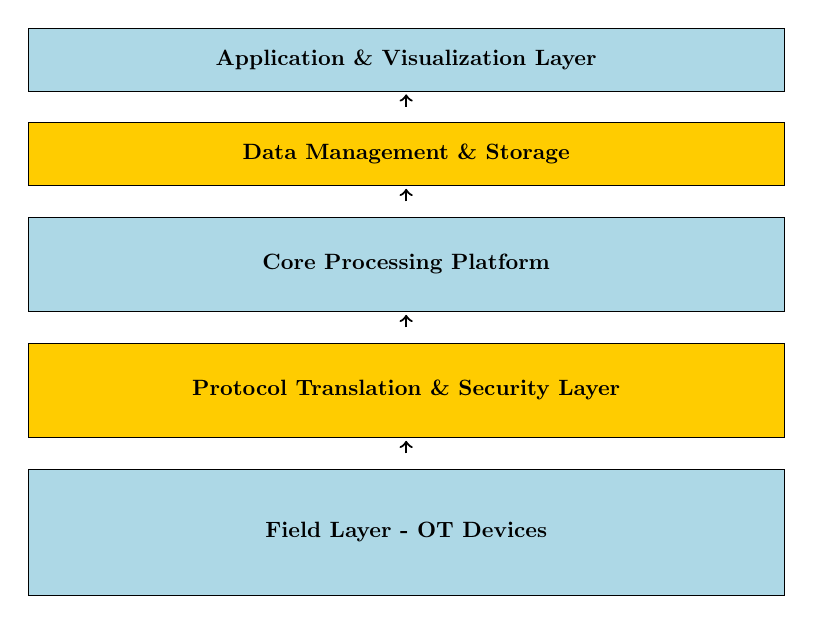
\begin{tikzpicture}[scale=0.8, transform shape]
% Draw main architecture layers
\draw[fill=lightblue] (0,0) rectangle (12,2);
\node at (6,1) {\textbf{Field Layer - OT Devices}};

\draw[fill=spitgold] (0,2.5) rectangle (12,4);
\node at (6,3.25) {\textbf{Protocol Translation \& Security Layer}};

\draw[fill=lightblue] (0,4.5) rectangle (12,6);
\node at (6,5.25) {\textbf{Core Processing Platform}};

\draw[fill=spitgold] (0,6.5) rectangle (12,7.5);
\node at (6,7) {\textbf{Data Management \& Storage}};

\draw[fill=lightblue] (0,8) rectangle (12,9);
\node at (6,8.5) {\textbf{Application \& Visualization Layer}};

% Add connecting arrows
\foreach \y in {2.25,4.25,6.25,7.75} {
    \draw[thick,->] (6,\y) -- (6,\y+0.2);
}
\end{tikzpicture}
\caption{AEGIS High-Level Architecture}
\end{figure}

\subsection{Core Modules Detail}

\subsubsection{AssetGuard - Intelligent Asset Discovery Engine}

AssetGuard employs advanced discovery techniques to automatically identify and catalog all OT assets within the network infrastructure.

\textbf{Key Features:}
\begin{itemize}
    \item Multi-protocol active \& passive scanning
    \item AI-powered device fingerprinting (99.5\% accuracy)
    \item Real-time topology mapping
    \item Vulnerability assessment integration
    \item Asset lifecycle management
\end{itemize}

\textbf{Technical Specifications:}
\begin{itemize}
    \item Discovery Speed: 10,000 devices/hour
    \item Protocol Support: 50+ industrial protocols
    \item Database: Neo4j graph database for relationships
    \item API: RESTful APIs for integration
    \item Accuracy: 99.5\% device identification rate
\end{itemize}

\subsubsection{ProtoSense - Universal Protocol Intelligence Platform}

ProtoSense provides comprehensive protocol analysis and anomaly detection across all supported industrial communication protocols.

\textbf{Architecture Components:}
\begin{table}[H]
\centering
\begin{tabular}{|p{3cm}|p{5cm}|p{6cm}|}
\hline
\rowcolor{lightblue}
\textbf{Component} & \textbf{Function} & \textbf{Technology} \\
\hline
Protocol Detector & Auto-identify protocols & Machine learning classification \\
\hline
Parser Factory & Generate protocol parsers & Template-based code generation \\
\hline
State Machine & Track protocol states & Finite state automaton \\
\hline
Validation Engine & Validate protocol semantics & Rule-based validation \\
\hline
Anomaly Detector & Detect protocol anomalies & Deep learning models \\
\hline
\end{tabular}
\caption{ProtoSense Component Architecture}
\end{table}

\subsubsection{ThreatHunter - AI-Powered Threat Detection System}

ThreatHunter leverages advanced machine learning algorithms to detect sophisticated cyber threats in OT environments.

\textbf{ML Model Pipeline:}
\begin{enumerate}
    \item \textbf{Data Ingestion:} Real-time stream processing (Apache Kafka)
    \item \textbf{Feature Engineering:} Automated feature extraction
    \item \textbf{Model Training:} Ensemble of ML algorithms
    \item \textbf{Inference Engine:} Real-time threat scoring
    \item \textbf{Alert Generation:} Priority-based alerting
\end{enumerate}

\textbf{Supported Threat Categories:}
\begin{itemize}
    \item Advanced Persistent Threats (APTs)
    \item Zero-day exploit detection
    \item Insider threat identification
    \item Supply chain compromise
    \item Ransomware detection
    \item Data exfiltration attempts
\end{itemize}

\subsubsection{ChainAudit - Blockchain-Powered Forensic System}

ChainAudit ensures tamper-proof logging and audit trail management using distributed ledger technology.

\textbf{Blockchain Architecture:}
\begin{table}[H]
\centering
\begin{tabular}{|p{3cm}|p{12cm}|}
\hline
\rowcolor{lightblue}
\textbf{Layer} & \textbf{Description} \\
\hline
Application Layer & Smart contracts for automated compliance and response \\
\hline
Consensus Layer & Practical Byzantine Fault Tolerance (PBFT) consensus \\
\hline
Network Layer & Permissioned network with role-based access \\
\hline
Data Layer & Merkle tree structure for efficient verification \\
\hline
\end{tabular}
\caption{ChainAudit Blockchain Architecture}
\end{table}

\subsubsection{DiodeGuard - Hardware-Accelerated Data Diode}

DiodeGuard provides unidirectional data transfer with guaranteed air-gap isolation for critical OT networks.

\textbf{Hardware Specifications:}
\begin{itemize}
    \item \textbf{Throughput:} 10 Gbps with <1ms latency
    \item \textbf{Optical Isolation:} Physical air-gap using optical transmission
    \item \textbf{Protocol Support:} Hardware-accelerated parsing for 50+ protocols
    \item \textbf{Security Certification:} FIPS 140-2 Level 3 compliance
    \item \textbf{Redundancy:} Dual-diode configuration with automatic failover
\end{itemize}

\textbf{FPGA Implementation Details:}
\begin{itemize}
    \item Xilinx Zynq UltraScale+ FPGA platform
    \item Custom protocol processing engines
    \item Hardware-based encryption/decryption
    \item Real-time packet inspection and filtering
    \item Dedicated security co-processors
\end{itemize}

\subsection{Advanced Technology Integration}

\subsubsection{Quantum-Resistant Cryptography}

AEGIS implements post-quantum cryptographic algorithms to ensure long-term security against quantum computing threats.

\textbf{Implemented Algorithms:}
\begin{itemize}
    \item \textbf{Lattice-based:} CRYSTALS-Kyber for key encapsulation
    \item \textbf{Hash-based:} SPHINCS+ for digital signatures
    \item \textbf{Code-based:} Classic McEliece for specific use cases
    \item \textbf{Multivariate:} Rainbow signatures for lightweight applications
\end{itemize}

\subsubsection{Zero-Trust Architecture for OT}

The platform implements a comprehensive zero-trust security model specifically designed for operational technology environments.

\textbf{Zero-Trust Principles:}
\begin{table}[H]
\centering
\begin{tabular}{|p{4cm}|p{8cm}|}
\hline
\rowcolor{lightblue}
\textbf{Principle} & \textbf{Implementation} \\
\hline
Never Trust, Always Verify & Continuous device and user authentication \\
\hline
Least Privilege Access & Role-based access control with minimal permissions \\
\hline
Assume Breach & Continuous monitoring and threat detection \\
\hline
Verify Explicitly & Multi-factor authentication and device attestation \\
\hline
\end{tabular}
\caption{Zero-Trust Implementation in AEGIS}
\end{table}

\newpage

\section{IMPLEMENTATION METHODOLOGY}

\subsection{Development Approach}

The AEGIS project follows an agile development methodology with security-by-design principles integrated throughout the development lifecycle.

\subsubsection{DevSecOps Pipeline}

\begin{figure}[H]
\centering
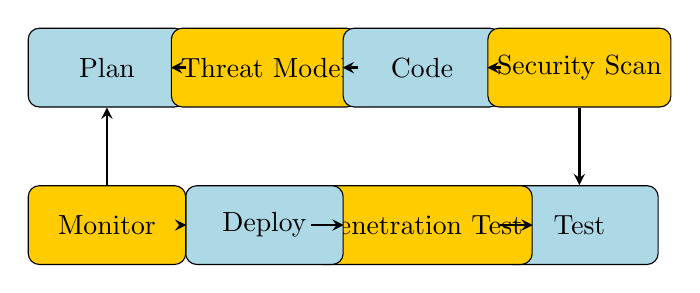
\begin{tikzpicture}[node distance=2cm, auto]
% Define styles
\tikzstyle{process} = [rectangle, rounded corners, minimum width=2cm, minimum height=1cm, text centered, draw=black, fill=lightblue]
\tikzstyle{security} = [rectangle, rounded corners, minimum width=2cm, minimum height=1cm, text centered, draw=black, fill=spitgold]
\tikzstyle{arrow} = [thick,->,>=stealth]

% Place nodes
\node [process] (plan) {Plan};
\node [security, right of=plan] (threat) {Threat Model};
\node [process, right of=threat] (code) {Code};
\node [security, right of=code] (scan) {Security Scan};
\node [process, below of=scan] (test) {Test};
\node [security, left of=test] (pentest) {Penetration Test};
\node [process, left of=pentest] (deploy) {Deploy};
\node [security, left of=deploy] (monitor) {Monitor};

% Draw arrows
\draw [arrow] (plan) -- (threat);
\draw [arrow] (threat) -- (code);
\draw [arrow] (code) -- (scan);
\draw [arrow] (scan) -- (test);
\draw [arrow] (test) -- (pentest);
\draw [arrow] (pentest) -- (deploy);
\draw [arrow] (deploy) -- (monitor);
\draw [arrow] (monitor) -- (plan);
\end{tikzpicture}
\caption{DevSecOps Pipeline for AEGIS Development}
\end{figure}

\subsubsection{Quality Assurance Framework}

\textbf{Testing Strategy:}
\begin{enumerate}
    \item \textbf{Unit Testing:} 95\% code coverage requirement
    \item \textbf{Integration Testing:} API and service integration validation
    \item \textbf{Performance Testing:} Load testing up to 1M events/second
    \item \textbf{Security Testing:} Automated vulnerability scanning
    \item \textbf{Penetration Testing:} Quarterly third-party security assessments
    \item \textbf{Compliance Testing:} Standards adherence verification
\end{enumerate}

\subsection{Project Timeline and Milestones}

\begin{figure}[H]
\centering
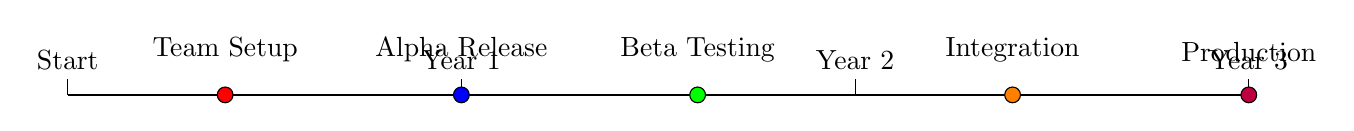
\begin{tikzpicture}
% Timeline
\draw[thick] (0,0) -- (15,0);

% Year markers
\foreach \x/\year in {0/Start, 5/Year 1, 10/Year 2, 15/Year 3} {
    \draw (\x,0) -- (\x,0.2);
    \node[above] at (\x,0.2) {\year};
}

% Milestones
\draw[fill=red] (2,0) circle (0.1);
\node[above] at (2,0.3) {Team Setup};

\draw[fill=blue] (5,0) circle (0.1);
\node[above] at (5,0.3) {Alpha Release};

\draw[fill=green] (8,0) circle (0.1);
\node[above] at (8,0.3) {Beta Testing};

\draw[fill=orange] (12,0) circle (0.1);
\node[above] at (12,0.3) {Integration};

\draw[fill=purple] (15,0) circle (0.1);
\node[above] at (15,0.3) {Production};

\end{tikzpicture}
\caption{Project Timeline with Key Milestones}
\end{figure}

\newpage

\section{RISK MANAGEMENT AND MITIGATION}

\subsection{Risk Assessment Matrix}

\begin{table}[H]
\centering
\caption{Project Risk Assessment Matrix}
\begin{tabular}{|p{4cm}|c|c|c|p{5cm}|}
\hline
\rowcolor{lightblue}
\textbf{Risk Category} & \textbf{Probability} & \textbf{Impact} & \textbf{Risk Level} & \textbf{Mitigation Strategy} \\
\hline

Technology Complexity & Medium & High & High & 
Incremental development, expert consultation, prototype validation \\
\hline

Talent Acquisition & High & Medium & High & 
Competitive compensation, academic partnerships, training programs \\
\hline

Integration Challenges & Medium & Medium & Medium & 
Standardized APIs, comprehensive testing, phased integration \\
\hline

Budget Overrun & Low & High & Medium & 
Detailed cost tracking, contingency planning, scope management \\
\hline

Timeline Delays & Medium & Medium & Medium & 
Agile methodology, parallel development tracks, risk buffers \\
\hline

Cybersecurity Threats & Low & High & Medium & 
Security-by-design, regular audits, incident response plans \\
\hline

\end{tabular}
\end{table}

\subsection{Quality Metrics and KPIs}

\textbf{Technical Performance Indicators:}
\begin{itemize}
    \item System throughput: ≥1M events/second
    \item Response latency: ≤100 milliseconds
    \item System availability: ≥99.99\%
    \item Threat detection accuracy: ≥99.5\%
    \item False positive rate: ≤0.1\%
\end{itemize}

\textbf{Project Management KPIs:}
\begin{itemize}
    \item Schedule adherence: ≥95\%
    \item Budget variance: ≤5\%
    \item Quality metrics: Zero critical defects
    \item Stakeholder satisfaction: ≥90\%
    \item Team productivity: 40 story points/sprint
\end{itemize}

\newpage

\section{EXPECTED OUTCOMES AND BENEFITS}

\subsection{Technical Deliverables}

\begin{enumerate}
    \item \textbf{Complete AEGIS Platform:} Production-ready cybersecurity solution
    \item \textbf{Source Code:} Full source code with documentation
    \item \textbf{Hardware Designs:} FPGA designs and hardware schematics
    \item \textbf{Patents:} 15+ patent applications filed
    \item \textbf{Research Papers:} 10+ publications in top-tier conferences
    \item \textbf{Training Materials:} Comprehensive certification programs
    \item \textbf{Test Environment:} Complete OT/IT test laboratory
\end{enumerate}

\subsection{Societal Impact}

\textbf{National Security Enhancement:}
\begin{itemize}
    \item Protection of critical infrastructure
    \item Reduced dependency on foreign cybersecurity solutions
    \item Enhanced cyber resilience for strategic industries
    \item Contribution to national cyber defense capabilities
\end{itemize}

\textbf{Economic Benefits:}
\begin{itemize}
    \item Direct job creation: 100+ high-skilled positions
    \item Indirect employment: 500+ jobs in supporting ecosystem
    \item Export potential: \rupees 1000\crores\ over 5 years
    \item Import substitution: \rupees 200\crores\ annually
    \item Cost savings: \rupees 500\crores\ from prevented cyber incidents
\end{itemize}

\textbf{Technology Leadership:}
\begin{itemize}
    \item Establishment of India as a global leader in OT cybersecurity
    \item Development of indigenous intellectual property
    \item Contribution to international standards and best practices
    \item Enhancement of India's reputation in cybersecurity research
\end{itemize}

\subsection{Knowledge Transfer and Capacity Building}

\textbf{Academic Partnerships:}
\begin{itemize}
    \item Collaboration with top Indian institutes (IITs, IISc, IIIT)
    \item Joint research programs and PhD thesis supervision
    \item Development of specialized cybersecurity curricula
    \item Industry-academia knowledge exchange programs
\end{itemize}

\textbf{Industry Training:}
\begin{itemize}
    \item Certification programs for cybersecurity professionals
    \item Hands-on training workshops for industry practitioners
    \item Development of specialized OT security competencies
    \item Creation of a skilled workforce for the cybersecurity sector
\end{itemize}

\newpage

\section{SUSTAINABILITY AND COMMERCIALIZATION PLAN}

\subsection{Business Model}

\textbf{Revenue Streams:}
\begin{enumerate}
    \item \textbf{Software Licensing:} Annual licensing for AEGIS platform
    \item \textbf{Hardware Sales:} Custom security hardware solutions
    \item \textbf{Professional Services:} Implementation and consulting services
    \item \textbf{Training and Certification:} Educational programs and certifications
    \item \textbf{Support and Maintenance:} Ongoing technical support services
    \item \textbf{International Licensing:} Technology licensing to foreign partners
\end{enumerate}

\subsection{Market Analysis}

\textbf{Target Market Segments:}
\begin{table}[H]
\centering
\begin{tabular}{|p{3cm}|p{3cm}|c|c|}
\hline
\rowcolor{lightblue}
\textbf{Segment} & \textbf{Market Size} & \textbf{Target Share} & \textbf{Revenue Potential} \\
& \textbf{(\rupees Cr)} & \textbf{(\%)} & \textbf{(\rupees Cr)} \\
\hline

Power \& Energy & 500 & 40 & 200 \\
\hline

Oil \& Gas & 300 & 30 & 90 \\
\hline

Manufacturing & 400 & 25 & 100 \\
\hline

Smart Cities & 200 & 50 & 100 \\
\hline

Transportation & 150 & 35 & 52.5 \\
\hline

Defense & 250 & 20 & 50 \\
\hline

\rowcolor{yellow}
\textbf{Total} & \textbf{1800} & \textbf{33} & \textbf{592.5} \\
\hline

\end{tabular}
\caption{Market Segmentation and Revenue Projections}
\end{table}

\subsection{Intellectual Property Strategy}

\textbf{Patent Portfolio:}
\begin{itemize}
    \item \textbf{Core Technologies:} 8 patents for fundamental innovations
    \item \textbf{Algorithm Patents:} 4 patents for AI/ML algorithms
    \item \textbf{Hardware Patents:} 3 patents for data diode technology
\end{itemize}

\textbf{Open Source Strategy:}
\begin{itemize}
    \item Release non-critical components as open source
    \item Contribute to existing open source security projects
    \item Build community around AEGIS platform
    \item Leverage open source for rapid adoption
\end{itemize}

\newpage

\section{BUDGET JUSTIFICATION}

\subsection{Capital Equipment Justification}

The capital equipment budget of \rupees 180\lakhs\ is essential for establishing a world-class research and development facility.

\textbf{High-End Computing Infrastructure (\rupees 95\lakhs):}
\begin{itemize}
    \item \textbf{GPU Servers:} Required for training complex AI/ML models for threat detection
    \item \textbf{High-Performance Servers:} Needed for real-time processing of 1M+ events per second
    \item \textbf{Storage Systems:} Essential for handling massive volumes of security data
    \item \textbf{Network Infrastructure:} Critical for high-throughput data processing
\end{itemize}

\textbf{Specialized Security Hardware (\rupees 35\lakhs):}
\begin{itemize}
    \item \textbf{Hardware Security Modules:} Required for cryptographic operations and key management
    \item \textbf{Custom Data Diodes:} Unique hardware for air-gapped security solutions
\end{itemize}

\textbf{Industrial Test Laboratory (\rupees 50\lakhs):}
\begin{itemize}
    \item \textbf{PLCs and RTUs:} Essential for testing with real industrial equipment
    \item \textbf{Smart Meters and PMUs:} Required for smart grid security research
    \item \textbf{Power System Simulators:} Critical for realistic testing scenarios
\end{itemize}

\subsection{Manpower Budget Justification}

The manpower budget of \rupees 210\lakhs\ over 3 years is allocated to attract and retain top-tier talent.

\textbf{Leadership Team (\rupees 60\lakhs):}
\begin{itemize}
    \item World-class project director with 20+ years of experience
    \item Proven track record in cybersecurity research and development
    \item International recognition and industry connections
\end{itemize}

\textbf{Technical Team (\rupees 120\lakhs):}
\begin{itemize}
    \item Senior engineers with specialized OT/IT security expertise
    \item PhD-level researchers for advanced algorithm development
    \item Hardware design experts for custom security solutions
\end{itemize}

\textbf{Support Team (\rupees 30\lakhs):}
\begin{itemize}
    \item Quality assurance and testing specialists
    \item Technical writers for comprehensive documentation
    \item Administrative support for project coordination
\end{itemize}

\newpage

\section{CONCLUSION}

The AEGIS project represents a transformative opportunity for India to achieve technological leadership in industrial cybersecurity. With the requested funding of \rupees 4.7 crores, this project will deliver:

\begin{enumerate}
    \item A world-class indigenous cybersecurity platform for critical infrastructure protection
    \item Significant contribution to national security and economic growth
    \item Development of cutting-edge technologies with global commercial potential
    \item Creation of a skilled cybersecurity workforce
    \item Establishment of India as a global leader in OT/IT security innovation
\end{enumerate}

The comprehensive technical approach, experienced team, and strong industry partnerships position AEGIS for success. The project's focus on practical implementation, combined with rigorous research methodology, ensures deliverable outcomes with real-world impact.

\textbf{Key Success Factors:}
\begin{itemize}
    \item \textbf{Technical Excellence:} Cutting-edge algorithms and hardware solutions
    \item \textbf{Industry Relevance:} Addresses real challenges in critical infrastructure
    \item \textbf{Scalable Architecture:} Designed for deployment across diverse environments
    \item \textbf{Strong Partnerships:} Government, industry, and academic collaboration
    \item \textbf{Commercial Viability:} Clear path to market adoption and sustainability
\end{itemize}

\textbf{Expected Return on Investment:}
\begin{itemize}
    \item \textbf{Direct ROI:} 250\% over 5 years through commercialization
    \item \textbf{Strategic Value:} Enhanced national security capabilities
    \item \textbf{Economic Impact:} \rupees 1500\crores\ in economic benefits
    \item \textbf{Technology Leadership:} Global recognition for Indian cybersecurity innovation
\end{itemize}

We respectfully request the Government of India's support for this critical national initiative that will establish India as a global leader in industrial cybersecurity while protecting our nation's most critical infrastructure assets.

\vspace{2cm}

\begin{center}
\textbf{"Securing India's Industrial Future, Today"}

\vspace{0.5cm}

\textbf{AEGIS - Where Innovation Meets Security}
\end{center}

\newpage

% Signatures and Contact Information
\section*{SIGNATURES AND CONTACT INFORMATION}

\vspace{1cm}

\begin{tabular}{p{7cm}p{7cm}}

\textbf{Principal Investigator:} & \textbf{Institute Head:} \\
\vspace{2cm} & \vspace{2cm} \\
\hrulefill & \hrulefill \\
Dr. [Name to be appointed] & Dr. [Director/Principal Name] \\
Principal Investigator \& Head & Director \\
Cybersecurity Research Division & SPIT, Mumbai \\
\textbf{Email:} pi.aegis@spit.ac.in & \textbf{Email:} director@spit.ac.in \\
\textbf{Phone:} +91-22-[Number] & \textbf{Phone:} +91-22-26707440 \\

\end{tabular}

\vspace{2cm}

\textbf{Institute Details:}
\begin{itemize}
    \item \textbf{Institution:} Bharatiya Vidya Bhavan's Sardar Patel Institute of Technology
    \item \textbf{Address:} Munshi Nagar, Andheri (West), Mumbai - 400058, Maharashtra, India
    \item \textbf{Website:} https://www.spit.ac.in
    \item \textbf{Email:} info@spit.ac.in
    \item \textbf{Phone:} +91-22-26707440
    \item \textbf{NAAC Grade:} A+ (Autonomous Status)
\end{itemize}

\vspace{1cm}

\textbf{Project Information:}
\begin{itemize}
    \item \textbf{Project Website:} https://aegis.spit.ac.in (to be created)
    \item \textbf{Technical Repository:} https://github.com/spit-aegis (to be created)
    \item \textbf{Documentation:} https://docs.aegis.spit.ac.in (to be created)
    \item \textbf{Project Email:} aegis@spit.ac.in
\end{itemize}

\vspace{1cm}

\begin{center}
\fbox{\begin{minipage}{0.8\textwidth}
\centering
\textbf{CERTIFICATE}

This proposal has been prepared in accordance with Government of India guidelines for R\&D project funding. All information provided is accurate and the institute commits to deliver the proposed outcomes within the specified timeline and budget.

\vspace{1cm}

\textbf{Date:} \today

\textbf{Place:} Mumbai, Maharashtra
\end{minipage}}
\end{center}

\end{document}
